In this section I will review current work in the area and place it in a spectrum with highly compatible on one side and highly complete on the other.
This culminates with Figure \ref{fig:Spectrum} at the end of this chapter that maps out the design space.

Most pointer-safety systems fall into one of three categories, based on how they track valid areas of memory.
In fat pointer systems, information about valid areas of memory is carried alongside the pointer, whereas in lookup table systems it is held seperate and associated with the pointer in some other method.
Finally, some systems use a poison based approach, where they signify areas of memory as being invalid and throw an error when an invalid area of memory is accessed.

\section{Systems requiring code rewrite}
Starting on the highly complete but poorly compatible end of the spectrum is Cyclone \cite{jim2002cyclone}, which is in fact a separate dialect of C.
Cyclone allows the programmer to write in a C-like language that is designed to prevent buffer overflows.
It does this by imposing restrictions, such as limiting pointer arithmetic and providing extensions, such as a never-null pointer type.
While some of these extensions are automatic, the programmer must make use of most of them explicitly which required between 0\% and 46\% of lines of code to be changed in the corpus tested.

Arguably other languages can be included in at this end of the spectrum. \textbf{A bit more}

\section{Systems requiring library recompilation}

The next step towards greater compatibility are systems that require the included libraries used by the program to be recompiled.
The library recompilation allows such systems to annotate or instrument the libraries, and deal intelligently with pointers returned from and sent to them.

CCured \cite{necula2002ccured} is primarily an analysis that annotates pointers with one of three types: \verb!SAFE! pointers which are only ever assigned to and dereferenced; \verb!SEQ! pointers that have pointer arithmetic performed on them and \verb!DYN! pointers which may have anything done to them including being cast from an integer.
Using this analysis, CCured can reduce the number of bounds checks that must be performed, however the analysis must be performed on the entire program, including libraries.
Coupled tightly with this analysis is a lookup table implementation of tracking bounds.

The Hardbound \cite{devietti2008hardbound} proposes hardware pointer checks and introduces the hardware bounded pointer. This is essentially a fat pointer, but the other fields are dealt with transparently by hardware.
All registers are upgraded to triples containing a value, base and bound, though the base and bound are set to zero for non-pointers.
It is suggested in the paper that Hardbound could be combined with CCured, where hardware bounded pointers are used to keep track of data about \verb!SEQ! and \verb!DYN! pointers.

The Intel Memory Protection Extensions \cite{mpx,intelMpxSpec} are a set of extensions to the x86 instruction set designed to check pointer references that may be exploited for security exploits.
They require compiler, runtime library and operating system support.

\section{Systems requiring program recompilation}

The Jones and Kelly bounds checker \cite{jones1997backwards} uses a table based approach, keeping a list of all objects in memory by tracking the uses of \verb!malloc! and \verb!free!.
This system holds a unique place in the compatibility to completeness scale, since it works with all programs written in standard compliant C, however an element of its transformation can break a non-standard but commonly used practice.

In standard C, pointers cannot point to an invalid memory address - they may only point to allocated memory addresses or one past the end of an array.
However, most implementations allow pointers to do this, and to maintain their (invalid) value, which may then be transformed to be valid again.
For example, the Ghostscript implementation of stacks uses pointers to the \verb!-1! element of an array.
The Jones and Kelly system however irrevocably invalidates such pointers.
Therefore, the Jones and Kelly bound checker requires the program to be rewritten if it does not adhere to the C standard.

In \textit{A Practical Dynamic Buffer Overflow Detector} \cite{ruwase2004practical} it was found that 60\% of programs tested did not adhere to the C-standard assumed in the Jones and Kelly approach and were therefore broken by the tactic of signifying illegal pointers by setting them to \verb!-2!.

To combat this, they created a new approach, where the creation of an out of bounds pointer would result in the creation of an Out Of Bounds object created on the heap which contains the address of the pointer and the referent object originally pointed to.
These Out Of Bounds objects are stored in a hash table.
Therefore on dereference, both the object list and the out of bounds hash table may be consulted to determine the validity of the pointer.
In order to reduce the overhead from these two lookups, only strings are bounds checked on the rationale that they are the tool used in buffer overflow attacks.

\textit{Baggy Bounds Checking} \cite{akritidis2009baggy} is an alternate optimization of the Jones and Kelly system, based on reducing the lookup time.
On a memory allocation, the size of the object is padded to the next power of two, enabling the size of the allocated memory to be stored more compactly as $lg_2(\mbox{size})$ taking the size of a single byte.
Due to the lower memory overhead of a entry, a constant sized array is used instead of an object list.
This allows a quick and constant time address calculation to be performed.
Alternate methods are used for dealing with pointers pointing past the end of arrays as adding one element to an array could double the size it could take up.

This approach does not prevent out of bounds accesses as the size associated with the pointer (the allocated bounds) is larger than the size of the object (the object bounds), so it is still possible to exceed the bounds of the object.
However it prevents dangerous overflows, since a pointer cannot access memory of an object that it was not created for.

LLVM's address sanitizer \cite{llvmAddrSan, llvmAddrSanAlgo} can be considered state of the art and  is capable of detecting out-of-bounds accesses on the heap, stack and for globals, use-after-free, and some use-after return bugs.

It does this by creating a copy of memory, called shadow memory, where 1 byte of shadow memory maps to 8 bytes of real memory.
This takes advantage of the fact that \verb!malloc! is guaranteed to return an 8-byte aligned segment of memory, therefore a value of 0 in shadow memory means the corresponding main memory is valid, a negative value means the corresponding main memory is invalid and a positive value of $n$ means the first $n$ bytes are valid and the rest are invalid.

The \verb!malloc! and \verb!free! functions are modified so as to mark the shadowed areas of memory as valid and poisoned respectively.
Additionally, \verb!malloc! is modified so that the memory surrounding that allocated to the program is poisoned to prevent overflows.

However, address sanitizer provides no mapping between the valid areas of memory and variables.
It would be possible for pointer arithmetic to be used to to still cause a buffer overflow into another variables' valid area of memory, though it must jump over the poisoned area.

One of the two main systems implemented in this dissertation is SoftBound \cite{nagarakatte2009softbound}.
It is a compile-time transformation that stores information about the valid area of memory associated with a pointer separately from the pointer.

By storing information separately from the pointer, memory layout doesn't change, enabling binary compatibility and reducing implementation effort, however it does require a search for suitable bounds information on pointer dereference.
Additionally the paper contains a proof that spatial integrity is provided by checking the bounds of pointers on a store or load.

\section{Systems requiring no recompilation}


\textit{Heapmon} \cite{shetty2005heapmon} deploys a helper thread that stores two bits for every word on the heap to keep track of whether or not the area is allocated and whether or not the area is initialized.
Memory leaks are therefore detected by looking for areas of allocated memory left over after the program exits.

To detect overflows, memory allocation is modified to leave unallocated areas between objects, so writing to that area will trigger an error.
Heapmon can only deal with memory on the heap (not the stack or globals) and works at a word granularity, so errors of less than 3 bytes may not be detected.

\textit{Body Armour for Binaries} \cite{slowinska2012body} targets a very specific type of attack - buffer overflows into non-control data, without requiring the source code or symbol table of the program.
It essentially does this by reverse engineering the binary to extract information about the data structures that need protecting and rewriting it to contain checks on pointer dereference.


\section{To Do}

\textit{Efficient Detection of all pointer and array access errors} \cite{austin1994efficient} uses a more complex fat pointer representation than just \{value, base, bound\} to extend their coverage beyond just spatial safety to include temporal safety.

The first additional field is the storage class enumeration, ranging over the values of Heap, Global and Local.
This allows detection of erroneous deallocations (such as attempting to free a local variable).
The second field, a capability is more interesting.
On memory allocation, a unique capability is created and stored in a capability table.
The capability is deallocated once the memory is freed (either through free or returning from a function).
The presence of the capability referenced by a fat pointer is checked on pointer dereference.
This was found to produce an overhead of between 130-450\%.


MPX

Lo-Pointers

CHERI

\section{Systems implemented in this Dissertation}

The fat pointer transformation implemented as part of Bandage is not a straight implementation from any research paper, but rather an implementation of the common themes spanning those that take the fat pointer approach.
The lookup table approach was more directly inspired by Softbound, using its lookup table structure (though with interchangeable implementations) and optimizations for dealing with local pointers.
Both of these transformations were designed with compatibility in mind, requiring a change only in the code for the program, not its libraries.

\section{Design Space}

\begin{figure}
\centering
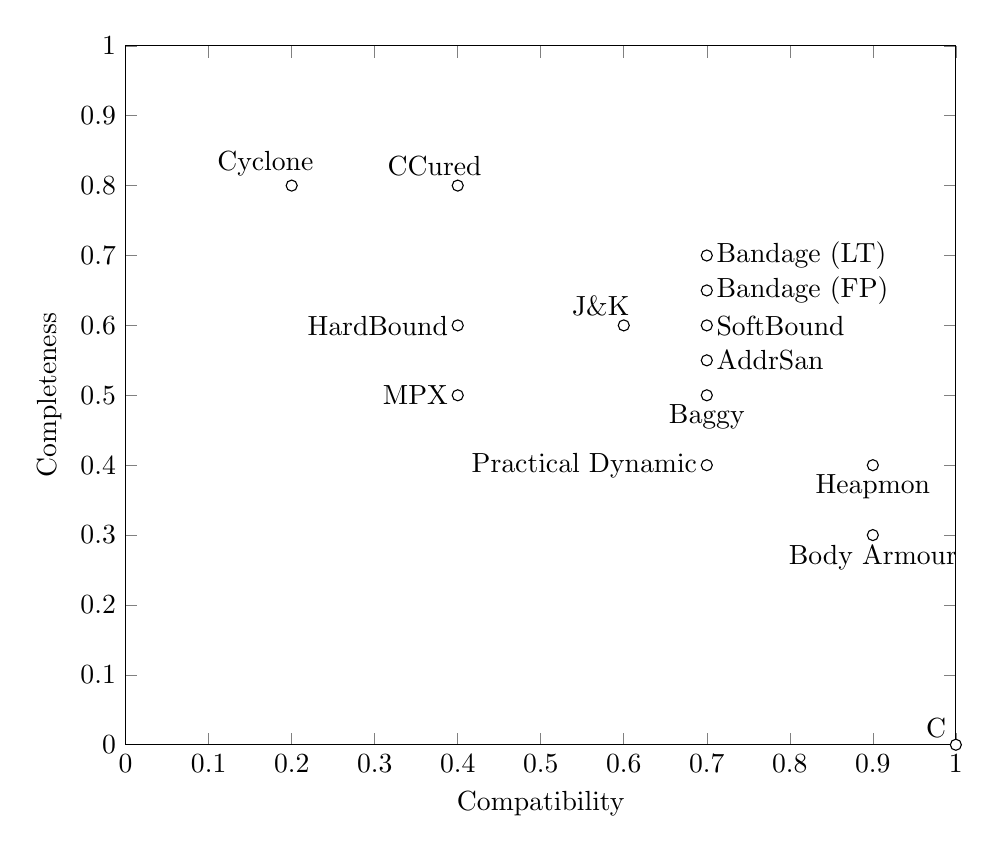
\begin{tikzpicture}
\begin{axis}[
    width=\textwidth,
    xmin=0,
    xmax=1,
    ymin=0,
    ymax=1,
    xlabel={Compatibility},
    ylabel={Completeness},
    ]
\addplot[
    only marks,
    mark=*,
    mark options={fill=white},
    visualization depends on=\thisrow{alignment} \as \alignment,
    nodes near coords, % Place nodes near each coordinate
    point meta=explicit symbolic, % The meta data used in the nodes is not explicitly provided and not numeric
    every node near coord/.style={anchor=\alignment}, % Align each coordinate at the anchor 40 degrees clockwise from the right edge
    ] table [% Provide data as a table
     meta index=2 % the meta data is found in the third column
     ] {
        x       y       label       alignment
        1       0       C           -40
        0.2     0.8     Cyclone     -40
        0.7     0.65     {Bandage (FP)}    180
        0.7     0.7     {Bandage (LT)}     180
        0.4     0.8     CCured      -40
        0.7     0.6     SoftBound   -180
        0.4     0.6     HardBound   0
        0.6     0.6     J\&K        -40
        0.9     0.4     Heapmon     90
	0.9	0.3	{Body Armour} 90
        0.7     0.55    AddrSan     180
        0.7     0.5     Baggy       90
	0.7	0.4	{Practical Dynamic} 0
        0.4     0.5     MPX         0
    };
\end{axis}
\end{tikzpicture}
\caption{The Completeness vs Compatibility Tradeoff in Pointer Safety Systems}
\label{fig:Spectrum}
\end{figure}

A summary of the design space is presented in Figure \ref{fig:Spectrum}.
At the very bottom end of completeness is the untransformed C language, which offers the highest compatibility but no pointer safety guarantees.
Offering the next step up in completeness are systems such as Heapmon and Body Armour for binaries which provide some protection without the need to recompile anything..

The completeness of a system is further increased by giving the system access to the programs source code and the ability to automatically instrument it, giving the myriad of tools forming the central region of the spectrum.
As the system becomes more integrated with the developer's toolchain, completeness increases, but the libraries need to be recompiled to work.
Finally, with Cyclone, the programmer assists the system in providing the most complete protection.
